\chapter{Background}\label{ch:background}

In this chapter, we will cover all the necessary theoretical background needed
in order to familiarize the reader with the rest of the document. We will
analyze the basic axis around that document, to avoid setting further
understanding difficulties to an unfamiliar with the subject reader.

More specifically, Section~\ref{sec:virt} covers the virtualization topic
since as we will see later, Ganeti is based on virtualization technologies.
Section~\ref{sec:cloud}, explains the term of Cloud Computing and how it is
evolved since it is first introduced in the computer science. Finally,
Section~\ref{sec:nosql} describes the new trend in the databases market,
the \emph{NoSQL} databases, as we used one of them to deal with some of Ganeti's
performance and scalability issues.

\section{Virtualization}\label{sec:virt}

In recent years, virtualization has become an important consideration and has
gained popularity in many different areas such as server consolidation, cloud
computing, corporate data centers, and the academic world. This is largely due
to an increase in hardware performance of about ten fold in the past decade, the
need to reduce the capital and operational cost to the minimum~\cite{Graziano},
and the desire to run multiple operating systems in a single host.

The term virtualization in computing, from a high level of view, refers to those
technologies designed to provide a logical view of computer resources, and
an abstraction layer between hardware systems and the software running
on them. Virtualization traces its roots back to the \emph{mainframes} of the
1960's and 1970's. There are various types of virtualization~\cite{virt_types},
and it can refer to a variety of computing concepts such as operating systems,
user-space applications, storage services, computer network resources, and more.
Maybe the most famous virtualization term is the \emph{Virtual Machine}. In the
early 1970's, Gerald J. Popek and Robert P. Goldberg defined the virtual machine
as:
\begin{flushright}
  \emph{``A virtual machine is taken to be an efficient,\\
        isolated duplicate of the real
        machine."}~\cite{DBLP:journals/cacm/PopekG74}


  Gerald J. Popek and Robert P. Goldberg
\end{flushright}
The definition of virtual machine has evolved since then, and current virtual
machine uses have not direct correspondence to any real hardware, necessarily,
and are used in a number of subdisciplines ranging from operating systems to
programming languages to processor architectures~\cite{smith_nair}. Depending on
the correspondence degree of a physical machine, virtual machines can be
classified into two major categories. The \emph{Process Virtual Machines} and
the \emph{System Virtual Machines}.

A \emph{process virtual machine} is a virtual platform that executes an
individual process in isolation from the physical computer system. It is often
called an \emph{application virtual machine} and its objective is to only
support the process it is assigned to. It is created and terminates as the
process is created and terminates respectively. This approach allows a user to
run a program that might otherwise be incompatible with the normal operating
system. The virtualization software that implements a process machine often
termed as \emph{``Runtime software"}. Such virtual machines are usually suited
to a programming language and build with the purpose of providing portability
and flexibility to the language. That type of VM has become popular since the
\emph{Java Virtual Machine (JVM)} introduction, used by the Java Programming
Language. They provide a high-level of abstraction and are implemented using an
interpreter to transform the instructions written in a specific programming
language into a machine language, which will run in the virtual environment
that the VM creates.

In contrast, a \emph{system virtual machine} provides a complete environment in
which an operating system with multiple users and many different processes can
coexist. With this type of VM, many different \emph{guest} operating systems
can run in a single \emph{host}, independently, isolated, and transparently from
each other. The guest operating system also provides access to virtual hardware
including network drivers, I/O communication, along with a virtual CPU (vCPU)
and memory. The software that implements a system virtual machine often referred
as the \emph{``Virtual Machine Monitor"}, VMM in short. These VMs usually
emulate an existing architecture, and are built with the purpose to provide a
platform for running programs when the real hardware is not available. In
addition, having multiple VM instances on a single host leads to a more
efficient use of computer resources, in terms of energy consumption and cost
effectiveness; the key that lead to the Cloud Computing evolution.

\subsection{Hardware Virtualization}

Hardware, or platform virtualization refers to the technique used
by the system virtual machines. In hardware virtualization, the
\emph{host} machine is the actual machine on which the virtualization takes
place, and the \emph{guest} machine is the virtual machine. The words host and
guest are used to distinguish the software that runs on the physical machine
from the software that runs on the virtual machine. VMs of that type use a
separate software layer called \emph{Hypervisor}. Hypervisor is the most basic
virtualization component and it is responsible for the creation and the
execution managing of the virtual machine. Hypervisors are classified on two
different types depending on running directly on the host's hardware,
\emph{Type I}, or running within a conventional OS environment, \emph{Type II}.

\emph{Type I} hypervisors, also called native or ``bare metal" ones, run
directly on the physical hardware, control it, and manage the guest operating
systems that run on a different level above the hardware, as Figure
\ref{fig:hypervisors} denotes. They are completely independent from the
operating system, and are also responsible for many basic operations like VM
scheduling, memory management, and more. They allow
multiple commodity operating systems run concurrently and share conventional
hardware in a safe way, but without sacrificing either performance or
functionality. Most known hypervisors of that type are the \emph{VMWare vShpere
Hypervisor}~\flink{http://www.vmware.com/products/vshpere-hypervisor/} and the
\emph{Xen Hypervisor}~\cite{xen_art}.

\emph{Type II} hypervisors, are running on top of a native operating system as a
separate distinct software layer, and below the guest's operating system, as
Figure~\ref{fig:hypervisors} presents. This type of hypervisor heavily
relies on the operating system, and is as secure as the OS itself.
On the other hand, a native operating system provides the ability to the
hypervisor to take advantage of the functions that are already implemented by
the OS, like scheduling, memory management, device drivers, and more.
The most known hypervisors of that category are the \emph{KVM}
hypervisor~\flink{http://www.linux-kvm.org/} which actually turns the Linux
kernel into a hypervisor, \emph{VirtualBox}~\flink{https://www.virtualbox.org/},
and the \emph{VMWare Workstation}
\flink{http://www.vmware.com/products/workstation/}.

\begin{figure}[htbp]
  \begin{center}
    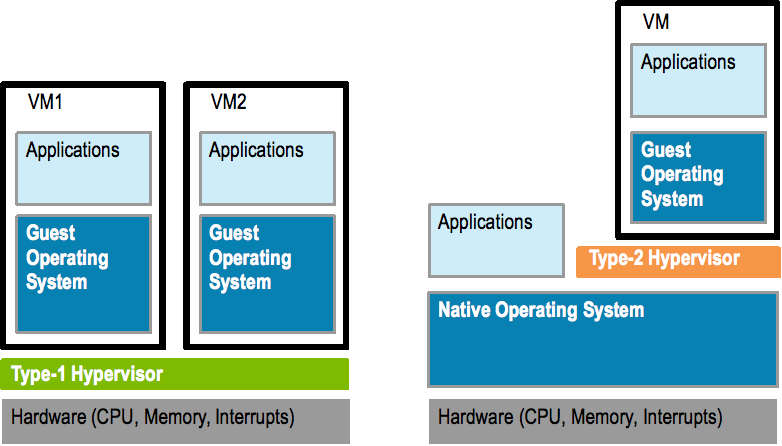
\includegraphics[width=0.8\maxwidth]{../figures/type1-vs-2.png}
    \caption{Hypervisor types\label{fig:hypervisors}}
   \end{center}
\end{figure}

Finally, we should mention another important hardware virtualization technique,
the \emph{Emulation}. It refers to the replication of system functions from
other, so that the emulator will act similarly to the emulated system.
\emph{QEMU}~\flink{http://www.wiki.qemu.org/} is maybe the most known hardware
emulator software, written by Fabrice Bellard~\cite{bellard}. It emulates central
processing units through dynamic binary translation, and provides a set of device
models, making it feasible to run a variety of unmodified guest operating systems.
It also provides an accelerated mode for supporting a mixture of binary
translation, for kernel code, and native execution, for user code, in the same
fashion as VMware Workstation and VirtualBox do. QEMU can also be used purely for
CPU emulation for user-level processes, allowing applications compiled for one
architecture to be run on another~\flink{http://en.wikipedia.org/wiki/QEMU}.

\subsection{Full Virtualization}

Full Virtualization is a hardware virtualization type on which the virtual
machine simulates almost completely the actual hardware to allow the guest
operating system software, mainly, to be run transparently and in isolation from
the rest system. That implies that every single feature of the physical hardware
can be reflected into a virtual machine, including interrupts, memory access,
and whatever other elements are used by the software that runs on the bare
machine.

Full virtualization is possible only with the right combination of hardware and
software elements. One of the most famous virtualization architectures
\emph{x86 architecture}~\cite{x86}, could not offer full virtualization until
the additions of the Intel VT-x
\flink{http://en.wikipedia.org/wiki/X86\_virtualization\#Intel\_virtualization\_.28VT-x.29}
and AMD-V
\flink{http://en.wikipedia.org/wiki/X86\_virtualization\#AMD\_virtualization\_.28AMD-V.29}
virtualization extensions, made at about 2005-2006. A key challenge for full
virtualization is the
interception and simulation of privileged operations, such as I/O instructions.
Every operation performed within a virtual machine should not affect other
virtual machines, or alter the state of the hardware. Many techniques have been
developed to provide the appearance of full virtualization. An interest approach
was implemented by VMware with a technique called \emph{``Binary translation"}
\cite{bin_tran}. We will not present further techniques because are
out of the scope of that document. \emph{KVM} and \emph{VMware} are well-known
examples of full virtualization solutions.

\subsection{Paravirtualization}

This technique does not simulates a hardware environment. However, the guest
applications are executed in their own isolated domains, as if they are running
on a separate system. With Paravirtualization the term of \emph{hypercall} is
introduced. The guest para-virtualized operating systems should make a system
call to the underlying hypervisor when it have to perform a privileged
operation. By allowing the guest OS to indicate its intents to the hypervisor,
improved performance and efficiency can be achieved, as each OS can cooperate to
obtain better performance when running in a virtual machine. As a result, the
guest OS have to be modified for the hypervisor, since the virtualization code
is integrated into the operating system itself. \emph{Xen} and \emph{User Mode
Linux} are examples of paravirtualization solutions.

\section{Cloud Computing}\label{sec:cloud}

Nowadays, the term \emph{Cloud} has become one of the most popular words
worldwide constituting a new trend in the computer science. Cloud Computing is
an overloaded term with many formulated definitions, which make us realize the
high interest of the topic. Although nearly everybody talks about cloud
computing, the concepts remain somewhat unclear to many, because a new
definition arises according to the field of interest. However, what we could say
about all the different definitions, is that they have in common the concept of
IT applications, infrastructures, and platforms provided on demand and
standardized as services over the Internet where the resources are provided to
the consumers logically rather than physically. According to that basic
understanding and based on our literature review we will try to provide a
definition from a computer resources perspective rather than a technical point
of view:

\begin{center}
  \emph{Cloud Computing is a design solution for an IT deployment, based on
        virtualized resources offered over the Internet, where its services in
        terms of infrastructure, software, storage, networking, and more, are
        offered on demand by a service provider, guaranteeing scalability,
        security, reliability and high-availability, and can be billed based on
        a per-usage paying policy.}
\end{center}

\subsection{The evolution of Cloud Computing}

Although the Cloud Computing became known to the public the last decade, that
does not constitutes a new invention or a revolution for the computer science.
It is more an evolution of already existing technologies rather than a new
computing paradigm. The following short historical review of the development of
computers and the Internet will show us that the idea of a centralized computer
utility was always existed and inevitably lead us to the beginning of Cloud
Computing~\cite{cloud_evolution}.

Going back in time we stop in \emph{1947}, the year when John Bardeen, Walter
Brattain, and William Shockley first introduced the \emph{transistor}. This is a
milestone in computer evolution because it marked great advancements in the
computer development. Computers evolved from simple calculating, Turing capable
to general-purpose machines~\footnote{Actually, \emph{ENIAC} (aka
Electronic Numerical Integrator And Computer), considered to be the first
general-purpose computer, which announced one year earlier in \emph{1946}, but
after \emph{1947} a burst in computer engineering occurs, with the first mass
produced computers.}. The underlying concept of cloud computing dates back in
late 1950s, when large-scale \emph{mainframe} computers become available in
academia and corporations. \emph{IBM 704}, in \emph{1954} was the first mass
produced mainframe computer with floating-point arithmetic. Eventually, in
\emph{1964} the \emph{IBM System/360} followed. Mainframe computers was
accessible via thin client/terminal computers. Primarily used by corporate
and governmental organizations for critical applications and bulk data
processing. The term originally referred to the large cabinets that housed the
central processing unit and the main memory of early computers. The peripheral
components that started to appear for that product family, in addition to
further developments and the miniaturization of the mainframes computers lead to
the appearance of \emph{Minicomputers}, such as \emph{DEC PDP-8}, in
\emph{1965}.

Mainframes were highly-costed computers. To make more efficient use of costly
mainframes, a practice evolved that allowed multiple users to share both the
physical access to computers from multiple terminals, as well as sharing their
CPU time. The practice of sharing the CPU time on mainframe computers, became
known in the
industry as \emph{time-sharing}. That trend of centralized, shared computer
resources is very similar to the idea of cloud computing. Many researchers in
the 1960ies talked about the need of computation to follow the electricity or
telephone system paradigm and be organized as a public
utility~\cite{cloud_imperative}.

\newpage
\begin{flushright}
  \emph{``Computing may someday be organized as a public utility just as the
         telephone system is a public utility ... Each subscriber needs to pay
         only for the capacity he actually uses, but he has access to all
         programming languages characteristic of a very large system ..."}


   Professor John McCarthy, at MIT’s centennial celebration in 1961
\end{flushright}

Douglas Parkhill's, \emph{1966} book, \emph{The Challenge of the Computer
Utility}, explores deeper this idea. With the \emph{Personal Computer (PC)}
development in the 1970ies significant performance leaps could be achieved,
graphical user interfaces were established, and the continuing miniaturization
eventually lead to the development of laptops and mobile devices. From
\emph{Intel 4004} first microprocessor in \emph{1971}, since \emph{1975 Altair
8800} first Home Computer, many PCs have been developed and even more followed
from Apple, IBM, and more companies that entered the industry.

In the \emph{1990ies}, the Internet achieved a real breakthrough with Tim
Berners-Lee's invention of the \emph{World Wide Web}. The concept of \emph{Grid
Computing} got established where a collection of computer resources from
multiple locations used to reach a common goal. The first appearance of the
term \emph{Cloud Computing}, happened at \emph{2007} some months after Amazon
made the test version of its \emph{Elastic Computing Cloud (EC2)} public. The
rapid development of \emph{Virtualization}, which allowed more efficient
hardware utilization made the cloud computing a technological innovation.
Nowadays more and more cloud solutions appear as mobile phones begin to overtake
PCs as the most common Web access devices worldwide.

The following Figure~\ref{fig:comp_evol}, gives us an overview of the computing
evolution.

\begin{figure}[htbp]
  \begin{center}
    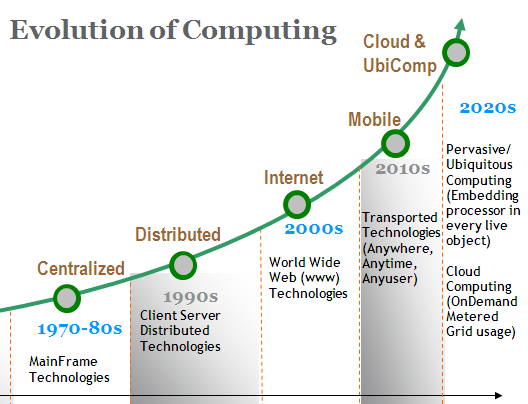
\includegraphics[width=0.75\maxwidth]{../figures/comp_evol.png}
    \caption{Computer history timeline\label{fig:comp_evol}}
   \end{center}
\end{figure}

\subsection{Service Models}

Cloud computing services can be classified along different layers, according to
the level of the capability they provide. There are three primary models, as
shown in Figure~\ref{fig:cloud_layers}, namely: Infrastructure as a Service
(\emph{IaaS}), Platform as a Service (\emph{PaaS}), and Software as a Service
(\emph{SaaS}). These abstraction levels can also be viewed as a layered
architecture where services of higher levels can be composed from the underlying
layers.

\begin{figure}[htbp]
  \begin{center}
    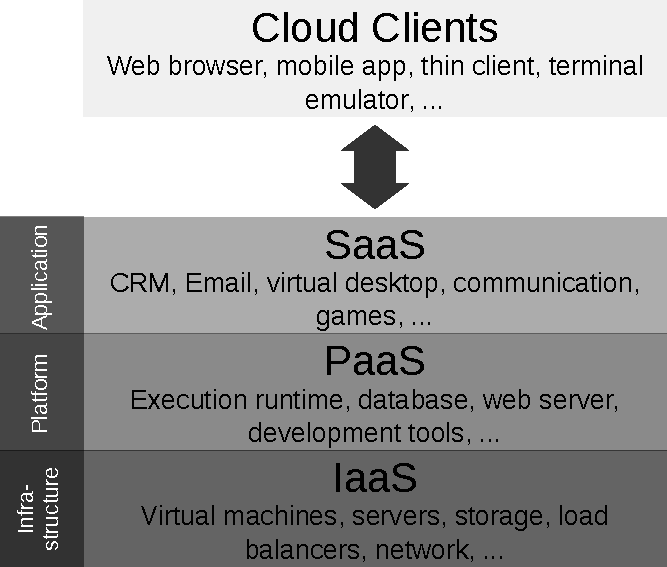
\includegraphics[width=1.0\maxwidth]{../figures/cloud_layers-black.pdf}
    \caption{The layers of Cloud Computing\label{fig:cloud_layers}}
   \end{center}
\end{figure}

\begin{description}
  \item[Infrastructure as a Service] \hfill \\
    It is the most basic cloud-service model. Providers of IaaS offer computers
    in terms of virtual machines, which are controlled by a hypervisor, such as
    Xen or KVM. Consumers can control and manage their systems in terms of
    operating systems, storage, applications, firewalls, and network connectivity
    but do not control the cloud infrastructure themselves. Examples of IaaS
    providers are the \emph{Amazon Web Services (AWS)}
    \flink{http://aws.amazon.com/}, Synnefo~\flink{http://www.synnefo.org/},
    Openstack~\flink{http://www.openstack.org/},
    Rackspace~\flink{http://www.rackspace.com/}, GoGrid~\flink{http://gogrid.com/}
    and more.
  \item[Platform as a Service] \hfill \\
    In the PaaS model, cloud providers offer a computing platform, typically
    including an operating system, a web server, a database and a programming
    language execution environment. Consumers purchase access to those platforms,
    enabling them to deploy their own software and applications in the cloud. The
    operating system or the network access are not managed by the consumers, which
    may have constraints on which applications they can deploy in the cloud. Some
    providers of a PaaS solutions are: Heroku~\flink{https://www.heroku.com/},
    Openshift~\flink{https://www.openshift.com/},
    AppFog~\flink{https://www.appfog.com/}, the Google App Engine
    Platform~\flink{https://developers.google.com/appengine/}, and many other.
  \item[Software as a Service] \hfill \\
    In that service model consumers purchase the ability to access and make use
    of application software and databases that are hosted in the cloud. Cloud
    providers manage the infrastructure and platforms that run the applications.
    SaaS can be referred as \emph{on-demand software} and is usually priced on a
    per-usage basis. The cloud users access the software most commonly from
    cloud clients. Salesforce~\flink{http://www.salesforce.com/} is the best
    known SaaS provider, which also considered to be the founder of the SaaS
    industry.
  \item[Other -aaS models] \hfill \\
    There are also many subsets of these models that are related to a more
    particular industry or market. Communication as a Service (\emph{CaaS}), is a
    model used to describe hosted IP telephony services. Network as a Service
    (\emph{NaaS}) provides network connectivity services and resource optimization
    allocations by considering network and computing resources as a unified
    whole. Database as a Service (\emph{DBaaS}), is another submodel offered
    by the cloud providers. As it seems, in coming years almost anything will
    be provided by the cloud as a service.
\end{description}

\subsection{Deployment Models}

Deploying cloud computing can differ depending on consumers requirements.
Four primary deployment models have been identified, each with specific
characteristics, used for several services and user needs.

\begin{description}
  \item[Private Cloud] \hfill \\
    The cloud infrastructure has been deployed, and is maintained and operated
    for a single organization. It can be hosted either internally or externally
    and managed internally or by a third-party.
  \item[Community Cloud] \hfill \\
    This deployment model is very similar to the private cloud, but the
    infrastructure is shared among several organizations with common interests
    and requirements. The cost for the cloud establishment is shared between
    organizations. The operation may be in-house or in third-party premises.
  \item[Public Cloud] \hfill \\
    The cloud infrastructure is available to the public by a service provider
    over the network. The most important technical difference compared to the
    private cloud is the security consideration, which can be considerably
    different depending on services like applications, storage, and more.
  \item[Hybrid Cloud] \hfill \\
    As it names stands for, hybrid cloud is a composition of two or more
    different cloud deployment models. The various cloud models which implement
    the hybrid one, are unique entities. The unified cloud instead, has the
    ability to communicate through its sub-cloud interfaces, allowing data or
    applications to be moved among
    them, and offering the benefits of multiple deployment models. Various use
    cases for hybrid cloud composition exist, like a combination of a
    public and private cloud that support both the requirement to retain some
    data in an organization, and also the need to offer some services in the
    cloud community.
\end{description}

\section{NoSQL databases}\label{sec:nosql}

Over the last 15 years, interactive applications have changed dramatically, and
so have the data management needs of those. The inception of Cloud Computing
gave higher priority to the application scalability, resource utilization, and
power saving. In addition to the growth in the global Internet usage, and the
growing popularity of smartphones and tablets, it is very common for applications
to have millions of users per day. Their usage requirements are
hard to predict, because user number rapidly grows or shrinks, and it is important
to dynamically support those differentiations. The large number of users created
the need of handling large amount of data, so databases should be able to
effectively deal with all this information~\cite{burd}.

The traditional SQL \emph{Relational DataBase Management Systems (RDBMS)}, based
on relational algebra~\flink{http://en.wikipedia.org/wiki/Relational\_algebra},
should be modified in order to meet up with the new requirements. At the beginning,
companies tried the traditional approach. Invested to more and faster hardware
as it became available. When that did not work, they tried to improve and make the
current relational models scale by simplifying the database schema, introducing
various caching layers, partitioning the data, and many more solutions in an
attempt to respond to the requirements of the new community that was
being developed. Although
each of these techniques extended the currently rigid database model and
addressed the core of the limitations that arose, they introduced additional
overhead to the applications. As a result, the previously optimal relational
database design, start to introduce limitations to the newly designed systems.
This is mainly due to the fact that when the majority of the relational
databases was designed, the predominant model for hardware deployment involved
buying large servers attached to storage area networks ,i.e., SANs. In other
words, the databases objective was to provide as much concurrent access as
possible with the given machine's limitations.

The common architecture of relational databases was the main reason that failed
to deal with scalability, latency, high-availability, failover options, speed,
fault-tolerance and other requirements of the largest sites during the massive
growth of the Internet. \emph{NoSQL} databases started to emerge, providing
solutions to the above requirements and in addition providing a great advantage;
agility. NoSQL designed and evolved in a different environment with different
needs and goals, and as a result provide better suited solutions for many of the
today's data storage
problems. Most agree that the term \emph{No}SQL, stands for \emph{``Not only"}
SQL, showing that the target is not to completely reject the existing relational
SQL models, but to overcome some of the limitations that exist. Database
architects sacrificed many primary aspects of the relational model, such as
joins or strong consistent data, while the schema devolved from strictly related
tables with primary/foreign key relations to something much more like a
key/value look up. Amazon's introduction of \emph{DynamoDB} and the underlying
paper~\cite{dynamo} considered by many the first large, web-scale production of
a NoSQL database.

\subsection{NoSQl compromises}

Companies want solutions that would scale, be fast, and operationally efficient.
They also ideally expect operations to speed up by simply adding new commodity
hardware, at almost a linear rate. One major bottleneck to accomplish that goal
are the database systems. So, in order to achieve the desired behavior, some
compromises should be made, and a bunch of tradeoffs should be taking into
account~\cite{burd}.

\begin{description}\label{item:cap}
  \item[The CAP Theorem] \hfill \\
    In \emph{2000}, Berkeley's CA researcher Eric Brewer published the CAP
    Theorem~\flink{http://en.wikipedia.org/wiki/CAP\_theorem}, also known as
    Brewer's Theorem. What Brewer claimed is that it is impossible for a
    distributed system to continually maintain perfect \emph{C}onsistency,
    \emph{A}vailability, and \emph{P}artition tolerance.

    \begin{itemize}
      \item \emph{Consistency}: All node see the same data at the same time.
      \item \emph{Availability}: A guarantee that every request receives a
            response about whether it was successful or failed.
      \item \emph{Partition tolerance}: The system will continue to operate
            despite arbitrary message losses.
    \end{itemize}

    The theorem states that when designing a database distributed system you
    must make tradeoffs among the above features because you cannot
    simultaneously maintain all three of them. Peter Mell, a senior computer
    scientist for the National Institute of Standards and Technology (NIST),
    said that:

    \begin{flushright}
      \emph{In the database world, they can give you perfect consistency, but
            that limits your availability or scalability. It’s interesting, you
            are actually allowed to relax the consistency just a little bit, not
            a lot, to achieve greater scalability.}

      \emph{Well, the big data vendors took this to a whole new extreme. They
            said that we are going to offer amazing availability or scalability,
            knowing that the data is going to be consistent eventually, usually.
            That was great for many things.}~\cite{peter_mell}
    \end{flushright}

    What Mell actually said is that maybe we need a balance. So systems should
    be developed with CAP tradeoffs, relative to operations that the product
    provides, rather than relative to the product as a whole. This is what a
    NoSQL solution actually does. It employs less constrained consistency models
    than traditional relational databases, but with higher availability and
    partition-tolerance.

  \item[ACID vs BASE] \hfill \\
    In computer science, \emph{ACID} is a set of properties which outlines the
    fundamental elements of transactions. In terms of database, a single
    logical operation on the data is called a transaction. ACID stands for
    Atomicity, Consistency, Isolation, and
    Durability~\flink{http://en.wikipedia.org/wiki/ACID}. In order to make a
    transaction more agile, and to deliver scalability, the NoSQL solutions
    should relax, or redefine some of those properties. Consistency and
    durability are the first ``runners".

    In distributed systems where there is a great deal of communication involving
    locks, scalability can not be easily achieved. One solution is to relax the
    consistency property and pass from \emph{``strong"} consistency to something
    called \emph{``eventual"} consistency. This actually means that updates made
    by a part of a
    system should become known to the rest parts of the system within a short
    period of time and not directly after the transaction is completed. For many
    applications the acknowledgment that the information will eventually arrive
    to all nodes satisfy the requirements. One other approach is using a concurrency
    control method called \emph{Multi Version Concurrency Control (MVCC)}
    \flink{http://en.wikipedia.org/wiki/Multiversion\_concurrency\_control}.
    Both of those techniques add an extra overhead to the programmer of
    the application who is responsible of dealing with the coming information
    appropriately. An another property is durability. Many NoSQL solutions
    choose not to save data to disk at once, because writing to disk slows down
    the whole system, but keeping them in memory instead. A balance should be
    found between durability and speed of performing read/write operations.
    Eventually, that approach keeps a small window open where seemingly committed
    transactions can be lost. Many other approaches designed, but as with any
    other databases, when evaluating a NoSQL solution, you should choose depending
    on your application requirements~\cite{burd}.

    The result of that \emph{``relaxing ACID"} approach followed by NoSQL
    solutions, characterized by the \emph{BASE} acronym:

    \begin{itemize}
      \item \emph{Basically Available}: By using data replication or sharding
            among many different servers, we result in a system that is always
            available, even if subsets of data become unavailable for short
            periods of time.
      \item \emph{Soft state}: In ACID systems, data consistency is one of the
            most painful requirements. On the other hand, NoSQL systems allow
            inconsistent data between nodes and leave that inconsistencies to
            the application developer.
      \item \emph{Eventually consistent}: In contrast with ACID systems that
            enforce consistency at transaction commit, NoSQL guarantees
            consistency only at some undefined future time.
    \end{itemize}

    Figure~\ref{fig:cap}, sums up everything discussed in the current subsection
    in a single image.

    \begin{figure}[htbp]
      \begin{center}
        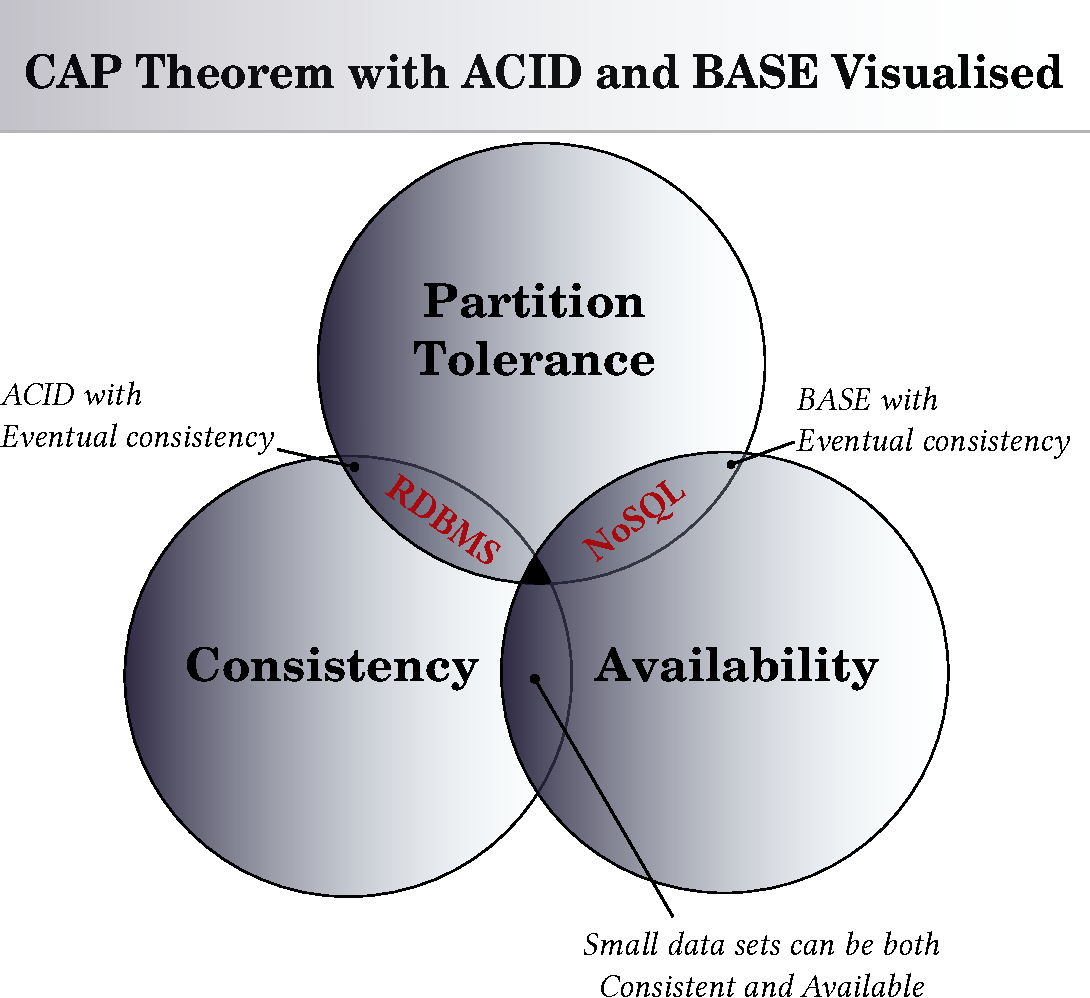
\includegraphics[width=0.8\maxwidth]{../figures/cap-nist.pdf}
        \caption{CAP theorem with ACID and BASE visualized\label{fig:cap}}
       \end{center}
    \end{figure}
\end{description}

\subsection{NoSQL Models}

Relational and NoSQL models are totally different. Relational models have rigid
schema which means that they require a strict definition of a schema prior to
storing any type of data into a database. Changing the schema once data are
inserted is a big deal, may be disruptive, and it is frequently avoided. In
addition, relational databases take data and separate them into many different
tables that contain rows and columns. Tables can be related through different
foreign keys that are stored in columns as well. A simple look up of a data,
requires a search among many tables and the subresults are combined before the
final answer can be provided to the application. Similarly, a write requires
data to be coordinated and performed on many different tables.

NoSQL databases follow a totally different approach. They are schema-less,
allowing to freely add fields without having to define the changes earlier.
The application
is not disrupted while the format of the data being inserted changes. They also
diverge from one another as well as from the RDBMS. There are three main
representation models within the NoSQL family:
Document-oriented, key/value, and graph
related databases. \emph{Key-value} databases allow the application to store its
data in a schema-less way. The data could be stored in a datatype of a
programming language or an object. Many different key/value types exist such as:
KV-eventual consistency, KV-cache in RAM, KV-solid state or rotating disk and
more. \emph{Document-oriented} database store data in formats that are more
native to the languages and systems they interact with. JSON or BSON, are
commonly used as a simple dictionary/array representation. \emph{Graph-based}
databases store information about nodes and edges and provide simple,
highly-optimized interface to examine the connections between them. We can
classify
NoSQL into more models like, Collection, or Columnar/Tabular oriented databases,
but we chose to present the three most known categories of them. In
Figure~\ref{fig:nosql_dbs}~\footnote{Source: \url{http://blog.nahurst.com/visual
-guide-to-nosql-systems}}, we present a bunch of the most known NoSQL
databases, and the models in which each one belongs, in combination with the CAP
theorem graph, to describe the various areas covered by each NoSQL database.

\begin{figure}[htbp]
  \begin{center}
    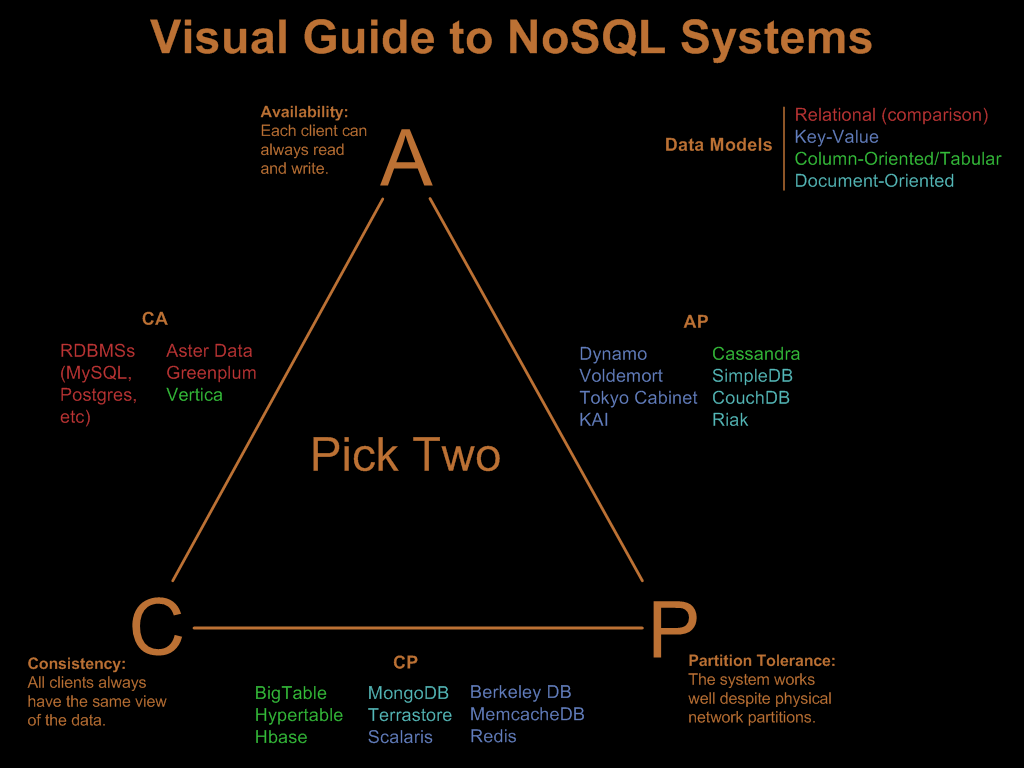
\includegraphics[width=1.0\maxwidth]{../figures/nosql_dbs.png}
    \caption{Visual guide to NoSQL systems\label{fig:nosql_dbs}}
   \end{center}
\end{figure}

NoSQL models have been designed with the intention to handle large amount of
data. Their main characteristics have been designed and developed
with respect to scaling and performance.
NoSQL solutions provide auto-sharding techniques. A NoSQL database automatically
spreads data across servers, without requiring application to participate.
Servers can be added or removed from the data layer without application
downtime. Most NoSQL databases also support data replication, storing multiple
copies of data across the cluster, or even more across data centers to ensure
high-availability and failover from hardware failures. In addition to
distributed data, they provide distributed processing techniques, mainly based on
MapReduce, providing them with powerful query capabilities even across hundred of
servers. Furthermore, to reduce latency and increase sustained data throughput,
advanced NoSQL database technologies transparently cache data in the system memory.
Summing up, NoSQL vs RDBMS debate will continue. Each has its advantages and
weaknesses, and neither will entirely replace the other. Spending some time on
understanding how the NoSQL tradeoffs will impact the application's design, may
result in a solution that fits the product's special needs, sometimes better
than a traditional RDBMS solution would.
